% Options for packages loaded elsewhere
\PassOptionsToPackage{unicode}{hyperref}
\PassOptionsToPackage{hyphens}{url}
\PassOptionsToPackage{dvipsnames,svgnames,x11names}{xcolor}
%
\documentclass[
  11pt,
  a4paper,
]{article}

\usepackage{amsmath,amssymb}
\usepackage{setspace}
\usepackage{iftex}
\ifPDFTeX
  \usepackage[T1]{fontenc}
  \usepackage[utf8]{inputenc}
  \usepackage{textcomp} % provide euro and other symbols
\else % if luatex or xetex
  \usepackage{unicode-math}
  \defaultfontfeatures{Scale=MatchLowercase}
  \defaultfontfeatures[\rmfamily]{Ligatures=TeX,Scale=1}
\fi
\usepackage{lmodern}
\ifPDFTeX\else  
    % xetex/luatex font selection
\fi
% Use upquote if available, for straight quotes in verbatim environments
\IfFileExists{upquote.sty}{\usepackage{upquote}}{}
\IfFileExists{microtype.sty}{% use microtype if available
  \usepackage[]{microtype}
  \UseMicrotypeSet[protrusion]{basicmath} % disable protrusion for tt fonts
}{}
\makeatletter
\@ifundefined{KOMAClassName}{% if non-KOMA class
  \IfFileExists{parskip.sty}{%
    \usepackage{parskip}
  }{% else
    \setlength{\parindent}{0pt}
    \setlength{\parskip}{6pt plus 2pt minus 1pt}}
}{% if KOMA class
  \KOMAoptions{parskip=half}}
\makeatother
\usepackage{xcolor}
\usepackage[top=2.4cm,bottom=2.4cm,left=2.5cm,right=2.5cm]{geometry}
\setlength{\emergencystretch}{3em} % prevent overfull lines
\setcounter{secnumdepth}{2}


\providecommand{\tightlist}{%
  \setlength{\itemsep}{0pt}\setlength{\parskip}{0pt}}\usepackage{longtable,booktabs,array}
\usepackage{calc} % for calculating minipage widths
% Correct order of tables after \paragraph or \subparagraph
\usepackage{etoolbox}
\makeatletter
\patchcmd\longtable{\par}{\if@noskipsec\mbox{}\fi\par}{}{}
\makeatother
% Allow footnotes in longtable head/foot
\IfFileExists{footnotehyper.sty}{\usepackage{footnotehyper}}{\usepackage{footnote}}
\makesavenoteenv{longtable}
\usepackage{graphicx}
\makeatletter
\def\maxwidth{\ifdim\Gin@nat@width>\linewidth\linewidth\else\Gin@nat@width\fi}
\def\maxheight{\ifdim\Gin@nat@height>\textheight\textheight\else\Gin@nat@height\fi}
\makeatother
% Scale images if necessary, so that they will not overflow the page
% margins by default, and it is still possible to overwrite the defaults
% using explicit options in \includegraphics[width, height, ...]{}
\setkeys{Gin}{width=\maxwidth,height=\maxheight,keepaspectratio}
% Set default figure placement to htbp
\makeatletter
\def\fps@figure{htbp}
\makeatother

\makeatletter
\@ifpackageloaded{caption}{}{\usepackage{caption}}
\AtBeginDocument{%
\ifdefined\contentsname
  \renewcommand*\contentsname{Table of contents}
\else
  \newcommand\contentsname{Table of contents}
\fi
\ifdefined\listfigurename
  \renewcommand*\listfigurename{List of Figures}
\else
  \newcommand\listfigurename{List of Figures}
\fi
\ifdefined\listtablename
  \renewcommand*\listtablename{List of Tables}
\else
  \newcommand\listtablename{List of Tables}
\fi
\ifdefined\figurename
  \renewcommand*\figurename{Figure}
\else
  \newcommand\figurename{Figure}
\fi
\ifdefined\tablename
  \renewcommand*\tablename{Table}
\else
  \newcommand\tablename{Table}
\fi
}
\@ifpackageloaded{float}{}{\usepackage{float}}
\floatstyle{ruled}
\@ifundefined{c@chapter}{\newfloat{codelisting}{h}{lop}}{\newfloat{codelisting}{h}{lop}[chapter]}
\floatname{codelisting}{Listing}
\newcommand*\listoflistings{\listof{codelisting}{List of Listings}}
\makeatother
\makeatletter
\makeatother
\makeatletter
\@ifpackageloaded{caption}{}{\usepackage{caption}}
\@ifpackageloaded{subcaption}{}{\usepackage{subcaption}}
\makeatother
\ifLuaTeX
  \usepackage{selnolig}  % disable illegal ligatures
\fi
\usepackage[style=authoryear-comp,]{biblatex}
\addbibresource{references.bib}
\usepackage{bookmark}

\IfFileExists{xurl.sty}{\usepackage{xurl}}{} % add URL line breaks if available
\urlstyle{same} % disable monospaced font for URLs
\hypersetup{
  pdftitle={Report of developing Learningtower R package},
  pdfauthor={Shabarish Sai Subramanian; Guan Ru, Chen},
  colorlinks=true,
  linkcolor={blue},
  filecolor={Maroon},
  citecolor={Blue},
  urlcolor={Blue},
  pdfcreator={LaTeX via pandoc}}

%% CAPTIONS
\usepackage{caption}
\DeclareCaptionStyle{italic}[justification=centering]
 {labelfont={bf},textfont={it},labelsep=colon}
\captionsetup[figure]{style=italic,format=hang,singlelinecheck=true}
\captionsetup[table]{style=italic,format=hang,singlelinecheck=true}

%% FONT
\usepackage{bera}
\usepackage[charter]{mathdesign}
\usepackage[scale=0.9]{sourcecodepro}
\usepackage[lf,t]{FiraSans}
\usepackage{fontawesome}

%% HEADERS AND FOOTERS
\usepackage{fancyhdr}
\pagestyle{fancy}
\rfoot{\Large\sffamily\raisebox{-0.1cm}{\textbf{\thepage}}}
\makeatletter
\lhead{\textsf{\expandafter{\@title}}}
\makeatother
\rhead{}
\cfoot{}
\setlength{\headheight}{15pt}
\renewcommand{\headrulewidth}{0.4pt}
\renewcommand{\footrulewidth}{0.4pt}
\fancypagestyle{plain}{%
\fancyhf{} % clear all header and footer fields
\fancyfoot[C]{\sffamily\thepage} % except the center
\renewcommand{\headrulewidth}{0pt}
\renewcommand{\footrulewidth}{0pt}}

%% MATHS
\usepackage{bm,amsmath}
\allowdisplaybreaks

%% GRAPHICS
\makeatletter
\def\fps@figure{htbp}
\makeatother
\setcounter{topnumber}{2}
\setcounter{bottomnumber}{2}
\setcounter{totalnumber}{4}
\renewcommand{\topfraction}{0.85}
\renewcommand{\bottomfraction}{0.85}
\renewcommand{\textfraction}{0.15}
\renewcommand{\floatpagefraction}{0.8}

%% SECTION TITLES
\usepackage[compact,sf,bf]{titlesec}
\titleformat*{\section}{\Large\sf\bfseries\color[rgb]{0.7,0,0}}
\titleformat*{\subsection}{\large\sf\bfseries\color[rgb]{0.7,0,0}}
\titleformat*{\subsubsection}{\sf\bfseries\color[rgb]{0.7,0,0}}
\titlespacing{\section}{0pt}{*5}{*1}
\titlespacing{\subsection}{0pt}{*2}{*0.2}
\titlespacing{\subsubsection}{0pt}{*1}{*0.1}

%% BIBLIOGRAPHY.

\makeatletter
\@ifpackageloaded{biblatex}{
\ExecuteBibliographyOptions{bibencoding=utf8,minnames=1,maxnames=3, maxbibnames=99,dashed=false,terseinits=true,giveninits=true,uniquename=false,uniquelist=false,doi=false, isbn=false,url=true,sortcites=false}
\DeclareFieldFormat{url}{\texttt{\url{#1}}}
\DeclareFieldFormat[article]{pages}{#1}
\DeclareFieldFormat[inproceedings]{pages}{\lowercase{pp.}#1}
\DeclareFieldFormat[incollection]{pages}{\lowercase{pp.}#1}
\DeclareFieldFormat[article]{volume}{\mkbibbold{#1}}
\DeclareFieldFormat[article]{number}{\mkbibparens{#1}}
\DeclareFieldFormat[article]{title}{\MakeCapital{#1}}
\DeclareFieldFormat[article]{url}{}
\DeclareFieldFormat[inproceedings]{title}{#1}
\DeclareFieldFormat{shorthandwidth}{#1}
\usepackage{xpatch}
\xpatchbibmacro{volume+number+eid}{\setunit*{\adddot}}{}{}{}
% Remove In: for an article.
\renewbibmacro{in:}{%
  \ifentrytype{article}{}{%
  \printtext{\bibstring{in}\intitlepunct}}}
\AtEveryBibitem{\clearfield{month}}
\AtEveryCitekey{\clearfield{month}}
\DeclareDelimFormat[cbx@textcite]{nameyeardelim}{\addspace}
\renewcommand*{\finalnamedelim}{\addspace\&\space}
}{}
\makeatother

%% PAGE BREAKING to avoid widows and orphans
\clubpenalty = 2000
\widowpenalty = 2000
\usepackage{microtype}% Placement of logos

\RequirePackage[absolute,overlay]{textpos}
\setlength{\TPHorizModule}{1cm}
\setlength{\TPVertModule}{1cm}
\def\placefig#1#2#3#4{\begin{textblock}{.1}(#1,#2)\rlap{\includegraphics[#3]{#4}}\end{textblock}}

% Title and date

\title{Report of developing Learningtower R package}
\date{25 October 2024}

\def\Date{\number\day}
\def\Month{\ifcase\month\or
 January\or February\or March\or April\or May\or June\or
 July\or August\or September\or October\or November\or December\fi}
\def\Year{\number\year}

%%%% PAGE STYLE FOR FRONT PAGE OF REPORTS

\makeatletter
\def\organization#1{\gdef\@organization{#1}}
\def\telephone#1{\gdef\@telephone{#1}}
\def\email#1{\gdef\@email{#1}}
\makeatother
  \organization{Department of Econometrics \& Business Statistics,
Monash University}

  \def\name{Department of\newline Econometrics \&\newline Business Statistics}

  \telephone{(03) 9905 2478}

  \email{BusEco-Econometrics@monash.edu}

\def\webaddress{\url{https://www.monash.edu/business/ebs}}
\def\abn{12 377 614 012}
\def\extraspace{\vspace*{1.6cm}}
\makeatletter
\def\contactdetails{\faicon{phone} & \@telephone \\
                    \faicon{envelope} & \@email}
\makeatother

\usepackage[absolute,overlay]{textpos}
\setlength{\TPHorizModule}{1cm}
\setlength{\TPVertModule}{1cm}

%%%% FRONT PAGE OF REPORTS

\def\reporttype{Report for}

\long\def\front#1#2#3{
\newpage
\begin{textblock}{7}(12.7,28.2)\hfill

\includegraphics[height=0.6cm]{AACSB}~~~

\includegraphics[height=0.6cm]{EQUIS}~~~

\includegraphics[height=0.6cm]{AMBA}
\end{textblock}
\begin{singlespacing}
\thispagestyle{empty}
\vspace*{-1.4cm}
\hspace*{-1.4cm}
\hbox to 16cm{
  \hbox to 6.5cm{\vbox to 14cm{\vbox to 25cm{
    
\includegraphics[width=6cm]{monash2}
    \vfill
    
\includegraphics[width=2cm]{MBSportrait}
    \vspace{0.4cm}
    \par
    \parbox{6.3cm}{\raggedright
      \sf\color[rgb]{0.00,0.00,0.70}
      {\large\textbf{\name}}\par
      \vspace{.7cm}
      \tabcolsep=0.12cm\sf\small
      \begin{tabular}{@{}ll@{}}\contactdetails
      \end{tabular}
      \vspace*{0.3cm}\par
      ABN: \abn\par
    }
  }\vss}\hss}
  \hspace*{0.2cm}
  \hbox to 1cm{\vbox to 14cm{\rule{1pt}{26.8cm}\vss}\hss\hfill}
  \hbox to 10cm{\vbox to 14cm{\vbox to 25cm{
      \vspace*{3cm}\sf\raggedright
      \parbox{10cm}{\sf\raggedright\baselineskip=1.2cm
         \fontsize{24.88}{30}\color[rgb]{0.70,0.00,0.00}\sf\textbf{#1}}
      \par
      \vfill
      \large
      \vbox{\parskip=0.8cm #2}\par
      \vspace*{2cm}\par
      \reporttype\\[0.3cm]
      \hbox{#3}%\\[2cm]\
      \vspace*{1cm}
      {\large\sf\textbf{\Date~\Month~\Year}}
   }\vss}
  }}
\end{singlespacing}
\newpage
}

\makeatletter
\def\maketitle{\front{\expandafter{\@title}}{\@author}{\@organization}}
\makeatother

% Authors

\author{\sf{\Large\textbf{Shabarish Sai Subramanian} \\\large Master of
Businss Analytics\\[0.5cm]}{\Large\textbf{Guan Ru, Chen} \\\large Master
of Businss Analytics\\[0.5cm]}}
\lfoot{\sf Subramanian, Guan Ru: 25 October 2024}
\begin{document}
\maketitle

\setstretch{1.5}
\section{Abstract}\label{abstract}

\section{Background}\label{background}

The learningtower package, which focusses on school and student-level
data like performance indicators, socioeconomic backgrounds, and
educational resources, contains educational datasets from international
exams like PISA before 2022. After being cleaned and standardised, these
datasets go through modifications including variable alignment for
consistency and student-teacher ratio calculations. Key performance
indicators include student performance in disciplines including reading,
mathematics, and science; school and country identities; and educational
resources (e.g., staff shortages, school size). The information makes it
possible to analyse regional and worldwide trends as well as differences
in educational systems, which sheds light on the variables influencing
resource allocation and academic performance.

\section{Introduction}\label{introduction}

A potent tool for analysing global educational data, the learningtower
program focusses on Programme for International Student Assessment
(PISA) statistics gathered over a number of years. These databases
include precise school and student-level statistics from several
nations, including student achievement in areas like reading,
mathematics, and science, as well as contextual aspects like school
resources, teacher-student ratios, and socioeconomic backgrounds. In
order to make data from prior years (before 2022) appropriate for
comprehensive cross-sectional and longitudinal investigations, the
package makes sure that the data is cleaned, standardised, and converted
to maintain consistency. With the help of this preparation, users can
investigate worldwide trends in education, spot inequalities, and
evaluate how various factors affect student achievements. We are now
integrating the 2022 dataset, which has been effectively configured
inside the package, guaranteeing that it is prepared for examination.
With this update, the package can now offer the most accurate and
up-to-date insights into global educational trends, allowing for greater
cross-country comparison and analysis.

\subsection{PISA}\label{pisa}

The Organization for Economic Cooperation and Development
\href{https://www.oecd.org/about/}{OECD} is a global organization that
aims to create better policies for better lives. Its mission is to
create policies that promote prosperity, equality, opportunity, and
well-being for all. \autocite{oecd}
\href{https://www.oecd.org/pisa/}{PISA} is one of OECD's Programme for
International Student Assessment. PISA assesses 15-year-old students'
potential to apply their knowledge and abilities in reading,
mathematics, and science to real-world challenges. OECD launched this in
1997, it was initially administered in 2000, and it currently includes
over
\href{https://www.oecd.org/pisa/aboutpisa/pisa-participants.html}{80
nations}. \autocite{pisa} The PISA study, conducted every three years,
provides comparative statistics on 15-year-old students' performance in
reading, math, and science. This report describes how to utilize the
\texttt{learningtower} package, which offers OECD PISA datasets from
2000 to 2022 in an easy-to-use format. The datasets comprise information
on students' test results and other socioeconomic factors, as well as
information on their schools, infrastructure and the countries
participating in the program.

\subsection{Learningtower Package}\label{learningtower-package}

\href{https://cran.r-project.org/web/packages/learningtower/index.html}{`learningtower'}
The R package \autocite{learningtower} provides quick access to a
variety of variables in the OECD PISA data collected over a three-year
period from 2000 to 2022. This dataset includes information on the PISA
test scores in mathematics, reading, and science. Furthermore, these
datasets include information on other socioeconomic aspects, as well as
information on their school and its facilities, as well as the nations
participating in the program.

The \texttt{learningtower} package primarily comprised of three
datasets: \texttt{student}, \texttt{school}, and \texttt{countrycode.}
The \texttt{student} dataset includes results from triennial testing of
15-year-old students throughout the world. This dataset also includes
information about their parents' education, family wealth, gender, and
presence of computers, internet, vehicles, books, rooms, desks, and
other comparable factors. Due to the size limitation on CRAN packages,
only a subset of the student data can be made available in the
downloaded package. These subsets of the student data, known as the
\texttt{student\_subset\_yyyy} (\texttt{yyyy} being the specific year of
the study) allow uses to quickly load, visualise the trends in the full
data. The full student dataset can be downloaded using the
\texttt{load\_student()} function included in this
\href{https://kevinwang09.github.io/learningtower/}{package.} The
\texttt{school} dataset includes school weight as well as other
information such as school funding distribution, whether the school is
private or public, enrollment of boys and girls, school size, and
similar other characteristics of interest of different schools these
15-year-olds attend around the world. The \texttt{countrycode} dataset
includes a mapping of a country/region's ISO code to its full name.

\section{Goals}\label{goals}

The motivation for developing the \texttt{learningtower} package was
sparked by the announcement of the PISA 2018 results, which caused a
collective wringing of hands in the Australian press, with headlines
such as
\href{https://theconversation.com/vital-signs-australias-slipping-student-scores-will-lead-to-greater-income-inequality-128301}{``Vital
Signs: Australia's slipping student scores will lead to greater income
inequality''} and
\href{https://www.smh.com.au/education/in-china-nicholas-studied-maths-20-hours-a-week-in-australia-it-s-three-20191203-p53ggv.html}{``In
China, Nicholas studied math 20 hours a week. In Australia, it's
three''}. That's when several academics from Australia, New Zealand, and
Indonesia decided to make things easier by providing easy access to PISA
scores as part of the \href{https://ozunconf19.ropensci.org/}{ROpenSci
OzUnconf}, which was held in Sydney from December 11 to 13, 2019.

The data from this survey, as well as all other surveys performed since
the initial collection in 2000, is freely accessible to the public.
However, downloading and curating data across multiple years of the PISA
study could be a time consuming task. As a result, we have made a more
convenient subset of the data freely available in a new R package called
\texttt{learningtower}, along with sample code for analysis.

\texttt{learningtower} developers are committed to providing R users
with data to analyse PISA results every three years. Our package's
future enhancements include updating the package every time additional
PISA scores are announced. Note that, in order to account for post
COVID-19 problems, OECD member nations and associates decided to
postpone the PISA 2021 evaluation to 2022 and the PISA 2024 assessment
to 2025.

\section{Compiling the data(more details about the process and problems
faced)}\label{compiling-the-datamore-details-about-the-process-and-problems-faced}

We are responsible for the curation of the newest PISA study, year 2022.
data on the participating students and schools were first downloaded
from the PISA website, in either SPSS or SAS format. The data were read
into an R environment. After some data cleaning and wrangling with the
appropriate script, the variables of interest were re-categorised and
saved as RDS files. One major challenge faced by the us was to ensure
the consistency of variables over the years. However, several variables
may be missing due to the reconstruction of questionnaires. For
instance, a question regarding student's possession of desk is not
recorded in 2022, but it was included in previous questionnaires, hence
these variables were manually curated as an character variable in the
output data. Another important issue we faced is a missing variable
\texttt{WEALTH}, this variable used to be a good measurement of a
student's socioeconomic status. But we also discovered a variable called
\texttt{ESCS} (economic, social and cultural status). These final RDS
file for each PISA year were then thoroughly vetted and made available
in a separate
\href{https://github.com/kevinwang09/learningtower_masonry}{GitHub
repository}.

\section{Communication and Documentation
Tools}\label{communication-and-documentation-tools}

Slack and Notion can be effectively utilized together to enhance team
communication and documentation management. Slack serves as a real-time
communication tool, allowing teams to quickly exchange information,
discuss projects, and stay updated on tasks, making it ideal for team
collaboration.

Notion, on the other hand, excels as a centralized workspace for
recording and organizing important documents, such as meeting journals,
project notes, and other key materials, ensuring that important
information is organized and easily accessible.

By using Slack for dynamic conversations and Notion for structured
documentation, teams can ensure seamless communication while maintaining
an organized record of all important documents, meeting notes, and
long-term planning.

\section{Overview of the data}\label{overview-of-the-data}

\subsection{Student Dataset}\label{student-dataset}

The dataset offers student-level information from a number of nations
and captures variables that affect academic performance. it contains the
23 variables, which could be categorized into groups:

\textbf{Year}*: represents the year of data collection, which is
manually constructed by the contributor.

\textbf{Country}: specifies the country from which the student data has
been collected, using country codes.

\textbf{School's inforamtion}: represents the unique identifier of each
student's school.

\textbf{Student's inforamtion}: This group provides some information
about each student in the dataset.

\begin{enumerate}
\def\labelenumi{\arabic{enumi}.}
\item
  \textbf{Parent's education}: record the parent's highest level of
  education based on the International Standard Classification of
  Education (ISCED) levels, ranging from ``less than ISCED1'' to ``ISCED
  3B, C''.
\item
  \textbf{Gender}: categorizes the gender of each student as ``male'' or
  ``female''.
\item
  \textbf{Household possession}: record several variables related to
  students' household resources. Including whether the student has
  access to a computer and internet at home, both marked as ``yes'' or
  ``no.'' Additional household resources are indicated by variables for
  a desk, separate room, dishwasher, television, and car. The number of
  computers and laptops is also available. Finally, the number of books
  in the student's home is categorized into ranges, such as ``0-10'' or
  ``101-200.
\item
  \textbf{Math, Read, Science}: These columns provide the scores in
  mathematics, reading, and science subjects, respectively.
\item
  \textbf{Stu\_Wgt}: Represents the student weight, used for calculating
  weighted averages in the analysis to ensure representative data.
\item
  \textbf{Wealth}: This column provides a measure of the student's
  economic wealth, where higher values indicate greater wealth. However
  this variable is not recorded in 2022 dataset.
\item
  \textbf{ESCS}: Represents the Economic, Social, and Cultural Status
  index, which is a composite measure of a student's socio-economic
  background.
\end{enumerate}

\subsection{School Dataset}\label{school-dataset}

The dataset includes school weight as well as other information such as
school funding distribution, whether the school is private or public,
enrollment of boys and girls, school size, and similar other
characteristics of interest of different schools these 15-year-olds
attend around the world.

\begin{verbatim}
# A tibble: 6 x 13
  year  country school_id fund_gov fund_fees fund_donation enrol_boys
  <fct> <fct>   <fct>        <dbl>     <dbl>         <dbl>      <dbl>
1 2000  ALB     01001          100         0             0       1191
2 2000  ALB     01004           98         1             1        334
3 2000  ALB     01005           91         5             2        403
4 2000  ALB     01010          100         0             0        114
5 2000  ALB     01013            0        50            30        250
6 2000  ALB     01017           95         2             3        771
# i 6 more variables: enrol_girls <dbl>, stratio <dbl>, public_private <fct>,
#   staff_shortage <dbl>, sch_wgt <dbl>, school_size <dbl>
\end{verbatim}

\begin{enumerate}
\def\labelenumi{\arabic{enumi}.}
\item
  \textbf{school\_id}: A unique identifier for each school, allowing for
  consistent tracking of school-related data across different records
  and years.
\item
  \textbf{public\_private}: Designates the type of school
  administration, distinguishing between public (government-funded) and
  private (independently funded) institutions.
\item
  \textbf{stratio}: Represents the student-teacher ratio, indicating the
  average number of students per teacher in the school. Lower ratios
  typically suggest smaller class sizes and potentially more
  individualized attention.
\item
  \textbf{staff\_shortage}: A measure indicating the level of staffing
  challenges faced by the school. Positive values may suggest severe
  shortages, while negative values or zeros may indicate minimal issues.
\item
  \textbf{school\_size}: The total number of students enrolled, which
  can reflect the school's capacity and influence on the learning
  environment. Larger schools may offer more diverse programs, while
  smaller ones might provide a more personalized setting.
\item
  \textbf{fund\_gov}: the percentage of funding that the government
  provides to the school. Understanding the resources available for
  staffing, programs, and infrastructure can be greatly aided by this.
\item
  \textbf{fund\_fees}: The proportion of money that came from student
  fees demonstrates the school's reliance on fee-based revenue, which is
  more usual in private institutions.
\item
  \textbf{fund\_donation}: represents the proportion of funds raised
  through donations, which could be a sign of extra support systems or
  community involvement.
\item
  \textbf{sch\_wgt}: In order to guarantee that the sample appropriately
  reflects the school population, school weight is utilised in
  statistical analysis, especially in weighted averages or survey data.
\end{enumerate}

\subsection{Countrycode Dataset}\label{countrycode-dataset}

This dataset includes a mapping of a country/region's ISO code to its
full name. More information on the participating countries can be found
\href{https://www.oecd.org/en/about/programmes/pisa/pisa-participants.html}{here}.

\section{Analysis}\label{analysis}

In this section we will illustrate how the \texttt{Learningtower}
package can be utilized to answer some research questions by applying
various methodologies and statistical computations on the
\texttt{Learningtower} datasets.

We will solely utilize the 2022 PISA data and scores for illustrative
purposes throughout the analysis section. Some of these questions
include if there is any significant gender difference between girls and
boys and explore their performance in the areas of mathematics, reading,
and science. Furthermore, we will inspect the various socioeconomic
characteristics reflected in the student data and investigate if they
have any substantial impact on the scores of these students.

\subsection{Gender Gap}\label{gender-gap}

Gender gaps have always been a topic of interest among researchers, and
when it comes to PISA data and scores of 15-year-old students around the
world, uncovering patterns based on their gender would help gain
meaningful insights in the field of education for various education
policymakers around the world. Based on the 2022 PISA results, let us
see if there is a major gender disparity between girls and boys
throughout the world in mathematics, reading, and science. To begin, we
will create a `data.frame' that stores the weighted average math score
for each nation as well as the various regions of the countries grouped
by country and gender, in order to create this \texttt{data.frame} and
represent data in the tidy format we use the \texttt{tidyverse}
\autocite{tidyverse} and \texttt{dplyr} \autocite{dplyr} R packages.
\href{https://www.oecd-ilibrary.org/education/pisa-2022-technical-report_01820d6d-en}{Survey
weights} are critical and must be used in the analysis to guarantee that
each sampled student accurately represents the total number of pupils in
the PISA population. In addition, we compute the gender difference
between the two averages. To demonstrate the variability in the mean
estimate, we use bootstrap sampling with replacement using the
\texttt{map\_dfr} function on the data and compute the same mean
difference estimate. For each country, the empirical 90 percent
confidence intervals are presented. The same process is used for reading
and science test scores.

\begin{figure}[H]

\centering{

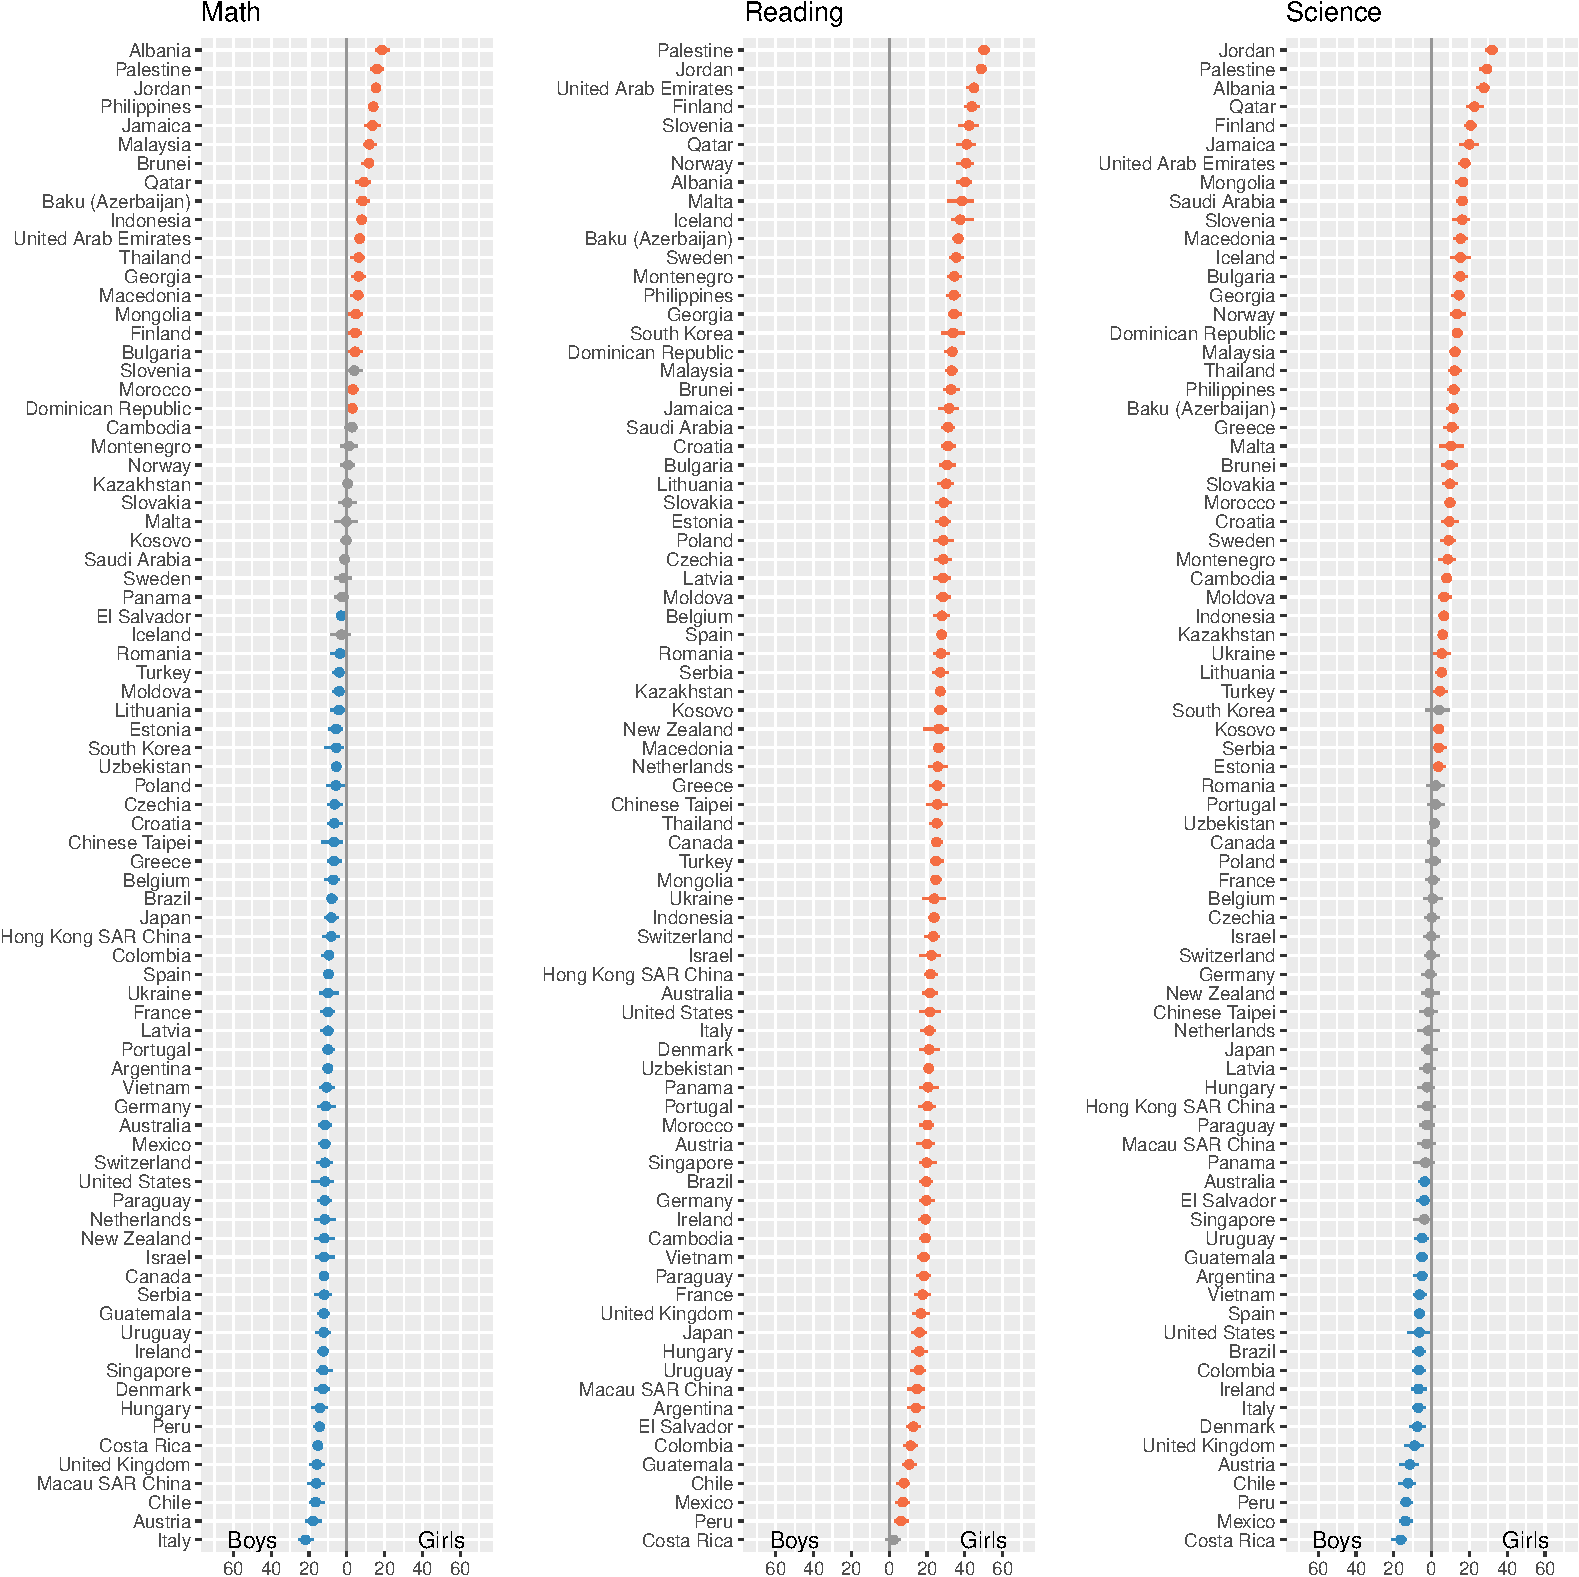
\includegraphics[width=1\textwidth,height=\textheight]{Learningtower_Rpackage_files/figure-pdf/fig-diff-1.pdf}

}

\caption{\label{fig-diff}The chart above depicts the gender gap
difference in 15-year-olds' in math, reading, and science results in
2022. The scores to the right of the grey line represent the
performances of the girls, while the scores to the left of the grey line
represent the performances of the boys. One of the most intriguing
conclusions we can get from this chart is that in the PISA experiment in
2022, girls from all countries outperformed boys in reading.The chart
above depicts the gender gap difference in 15-year-olds' in math,
reading, and science results in 2022. The scores to the right of the
grey line represent the performances of the girls, while the scores to
the left of the grey line represent the performances of the boys. One of
the most intriguing conclusions we can get from this chart is that in
the PISA experiment in 2022, girls from all countries outperformed boys
in reading.}

\end{figure}%

Figure~\ref{fig-diff} illustrates the global disparities in mean math,
reading, and science outcomes, before we get to the plot conclusion,
let's have a look at the variables that have been plotted. The grey line
here indicates a reference point, and all of the scores to the right of
the grey line show the scores of girls in math, reading, and science.
Similarly, the scores on the left side of this grey line indicate the
scores of boys in the three disciplines. Based on Figure~\ref{fig-diff},
because most math estimates and confidence intervals lie to the left of
the grey line, we may conclude that most boys outperformed girls in
math.

In nations such as Panama, Malta, Saudi Arabia, Sweden, Kazakhstan,
Norway, Slovenia, Iceland, Kosovo, Cambodia, Montenegro and Slovakia,
there is almost no gender difference in average math scores. When we
look at the reading scores, we notice a remarkable trend in that all
girls outpaced boys in reading in all countries in 2022. The highest
reading scores were achieved by girls from Palestine, Jordan and United
Arab Emirates. Looking further into the science plot, we see an
unexpected pattern here where most countries have very little gender
difference in science scores, implying that most boys and girls perform
equally well in science. Boys from Costa Rica, Mexico and and Peru
perform well in science and girls from Jordan, Palestine, and Albania
are the top scores for science. Figure~\ref{fig-diff} helps us to depict
the gender gap in math, reading, and science for all nations and regions
that took part in the 2022 PISA experiment.

We gathered meaningful insights about the gender gap between girls and
boys across the world from the above Figure~\ref{fig-diff} because this
is a geographical research communication topic, the findings will help
us better comprehend the score differences in the three educational
disciplines using world maps. Let us continue to investigate and
discover patterns and correlations using map visualization. To
illustrate the gender gap difference between girls and boys throughout
the world, we summarize regions on a country level and utilize the
\texttt{map\_data} function to get the latitude and longitude
coordinates needed to construct a map for our data. We connect these
latitude and longitude coordinates to our PISA data and render the world
map using the \texttt{geom\_polygon} function wrapped within
\texttt{ggplot2} \autocite{ggplot2}, the interactive features and
placement of the plots are made using \texttt{plotly} \autocite{plotly}
and \texttt{patchwork} \autocite{patchwork} packages in R.

\begin{figure}[H]

\centering{

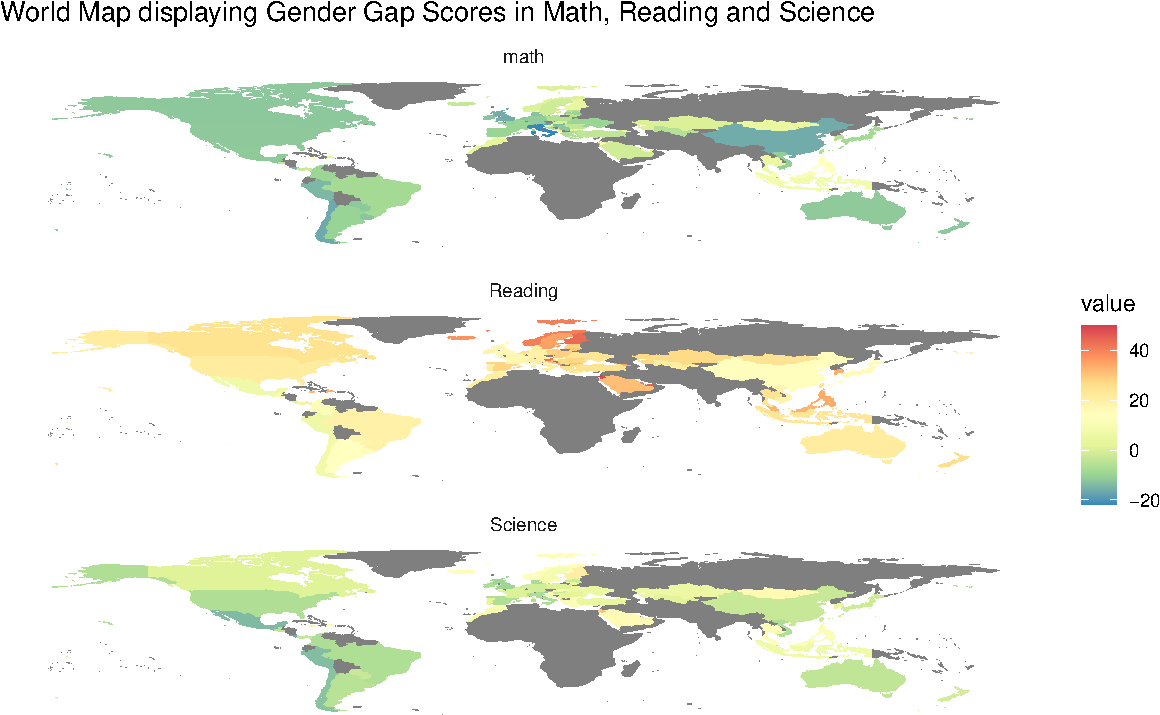
\includegraphics[width=1\textwidth,height=\textheight]{Learningtower_Rpackage_files/figure-pdf/fig-worldmaps-1.pdf}

}

\caption{\label{fig-worldmaps}Maps showing the gender gap in math,
reading, and science results between girls and boys across the world. A
positive score for a country indicates that girls outperformed boys in
that country, whereas a negative score for a country difference
indicates that boys outperformed girls in that country. The diverging
colour scale makes it possible to interpret the range of scores and the
also helps us intrepret the gender gap difference among these students
across the globe.}

\end{figure}%

In the Figure~\ref{fig-worldmaps}, we have shown the gender gap
difference between girls and boys in math, reading, and science in 2022.
Map visualization aids in the comprehension of large volumes of data in
a more efficient manner and increases the ability to compare outcomes
across many geographical locations at a glance. In this figure, we see
both positive and negative score difference scale ranges in all three
maps. A positive country score indicates that girls outperformed boys in
that country, whereas a negative country score shows that boys outscored
girls in that country. The diverging spectral color scale and the legend
of these maps makes it possible for us to deduce and identify regions
across the globe showing large gender discrepancy between girls and
boys. The grey colour for different geographic locations across the maps
in Figure~\ref{fig-worldmaps} indicates that these regions were not a
part of the PISA experiment in year 2022.

Even though the map visualization embeds the same scores as
Figure~\ref{fig-worldmaps}, one of the most striking thing on this map
is the lack of data for the Africa continent. We see that there is less
of a gender disparity seen in the science scores compared to maths and
reading. In addition, the color scale for scores of each subject aids in
identifying the countries that took part in the PISA experiment. As a
result, in this section, we have seen the gender gap scores and striking
trends between 15-year-old girls and boys in math, reading, and science.
Our main conclusion from this gender study is the performance of girls
in reading. The fewer gender disparity is evident in the science scores,
and the majority of boys perform better than girls in mathematics.

\subsection{EcoSocio factors}\label{ecosocio-factors}

\begin{figure}[H]

\centering{

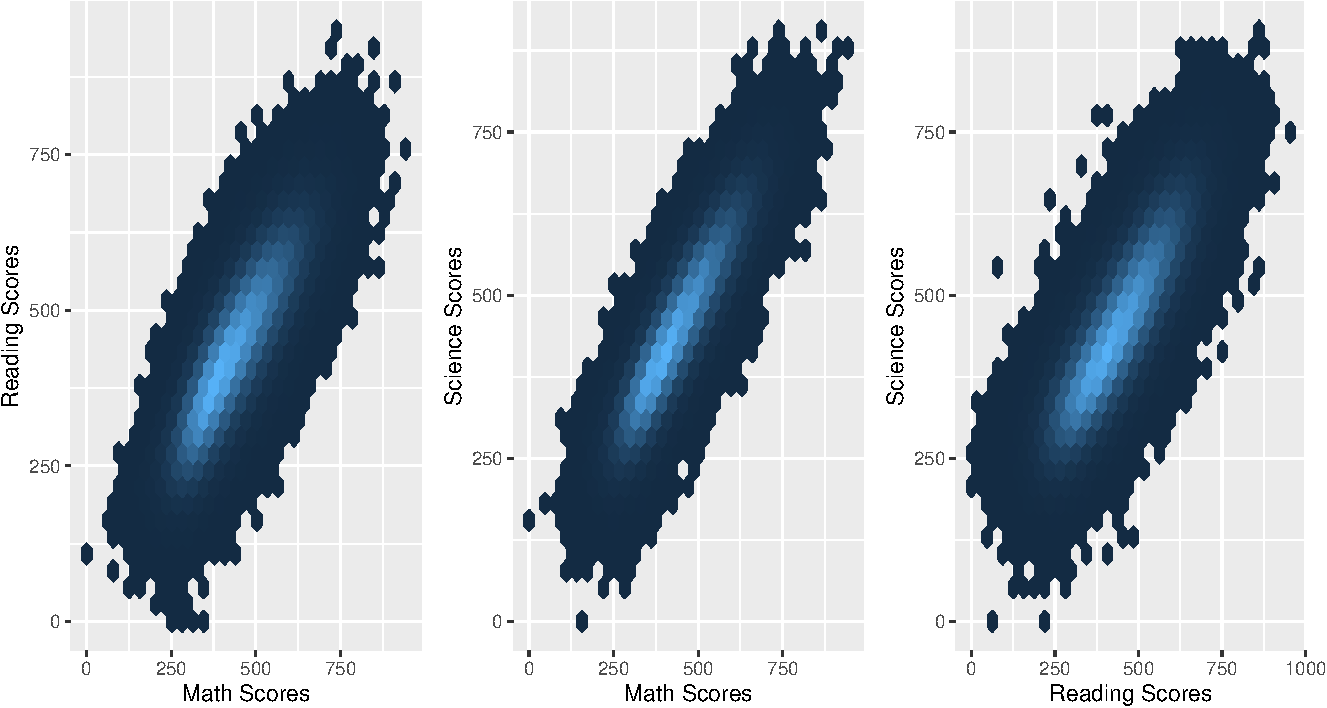
\includegraphics[width=1\textwidth,height=\textheight]{Learningtower_Rpackage_files/figure-pdf/fig-corrplot-1.pdf}

}

\caption{\label{fig-corrplot}The scatterplot displays the relationship
between math, reading, and science scores for all PISA countries that
participated in the experiment in 2022. This scatterplot shows that all
three subjects have a significant and positive correlation with one
another.}

\end{figure}%

\begin{figure}[H]

\centering{

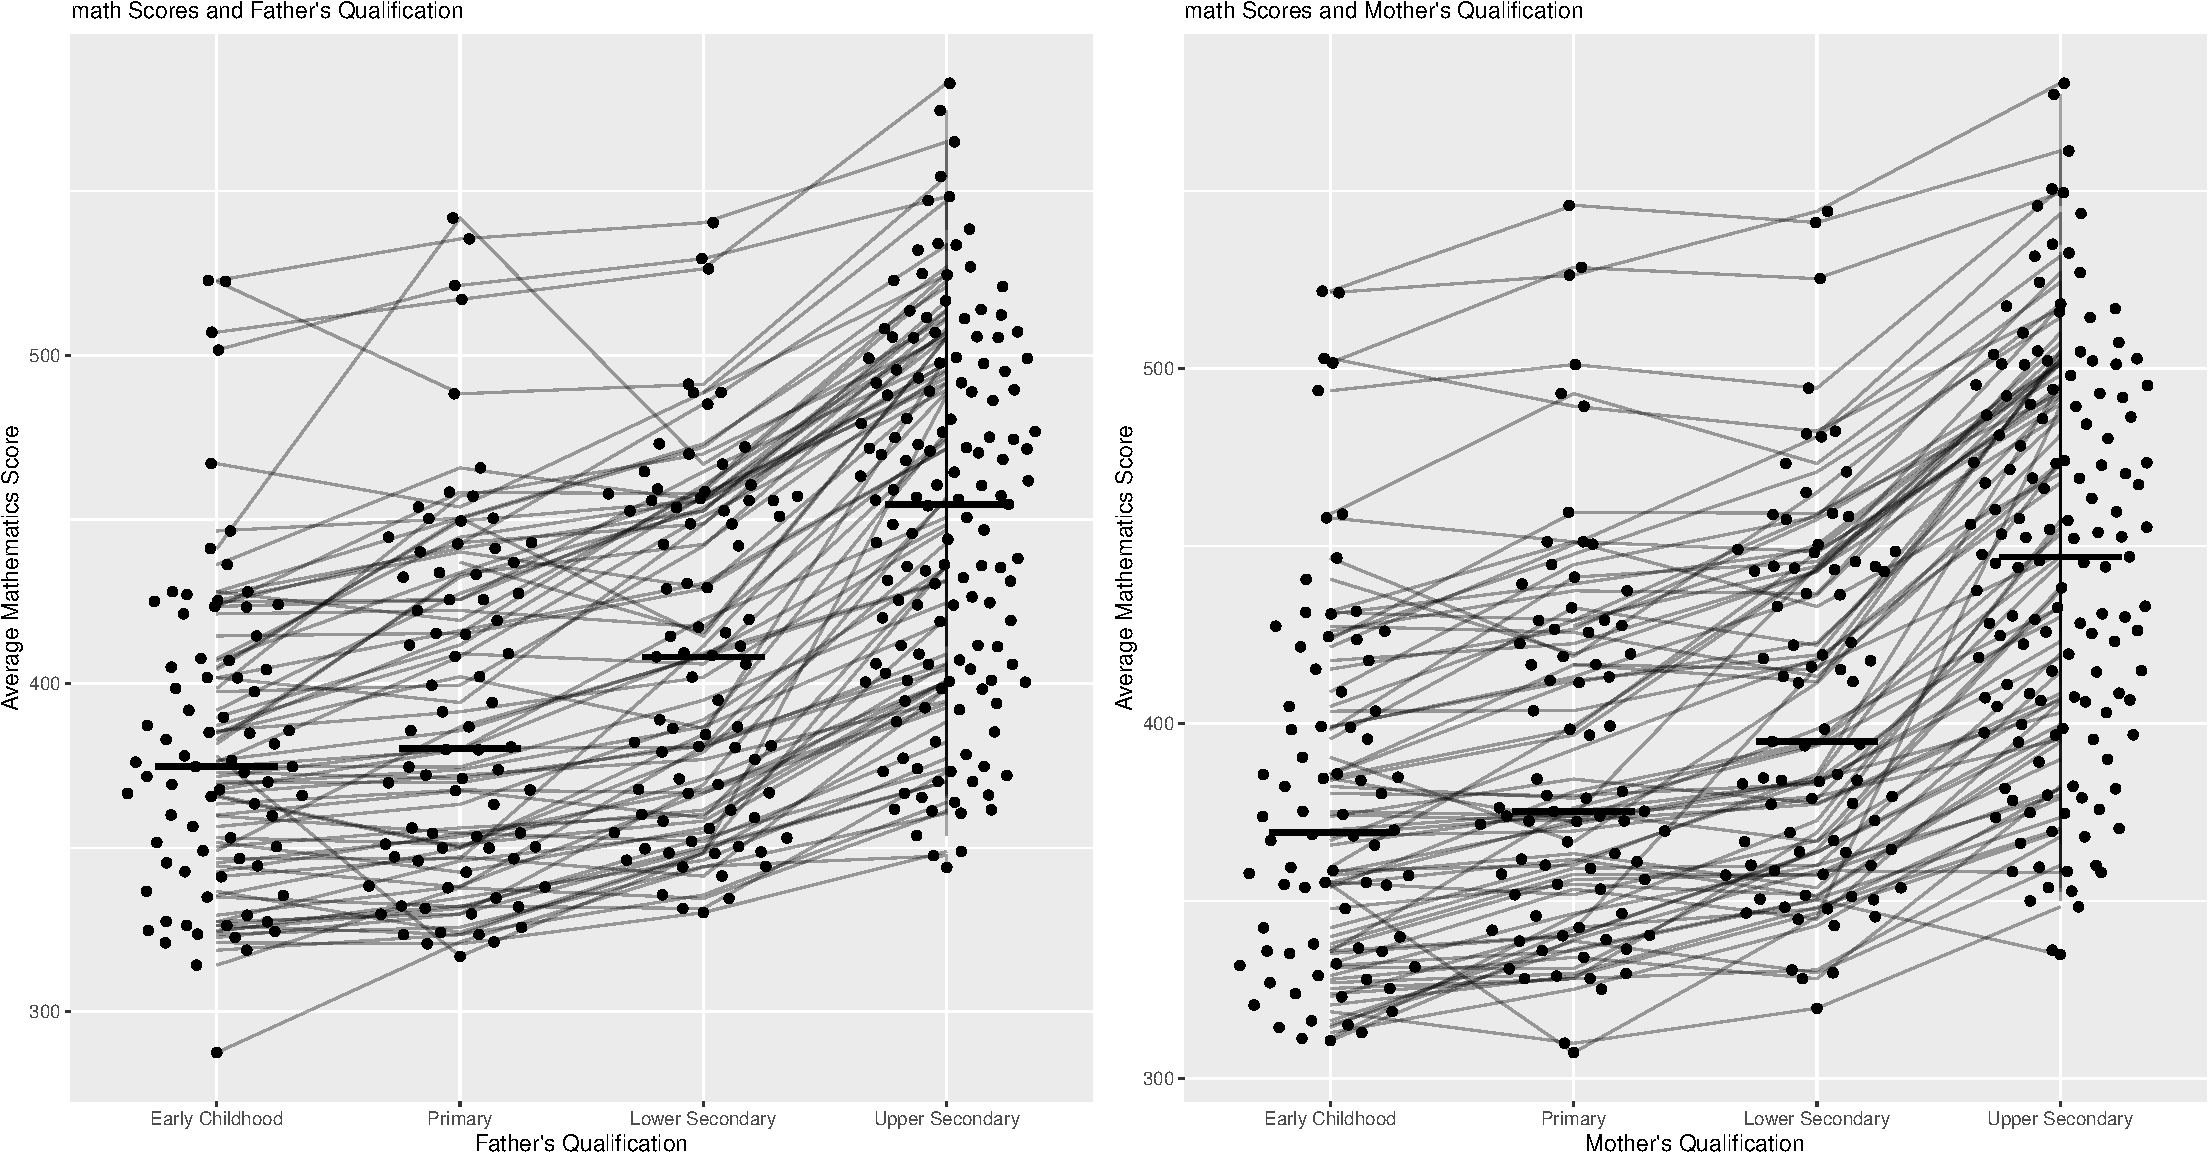
\includegraphics[width=1\textwidth,height=\textheight]{Learningtower_Rpackage_files/figure-pdf/fig-qualplot-1.pdf}

}

\caption{\label{fig-qualplot}The impact of parents' education on their
children's academic progress is depicted in this graph. When the parents
have greater levels of education, we see a considerable rise in scores
and an increase in the median of scores for each category, as shown in
the figure. In comparison to parents with lower levels of education
qualifications. Parents who have tend to have upper secondary
qualification or equivalent credentials their children are more likely
to perform better in academics when compared with parent having lesser
levels of qualifications.}

\end{figure}%

\begin{figure}[H]

\centering{

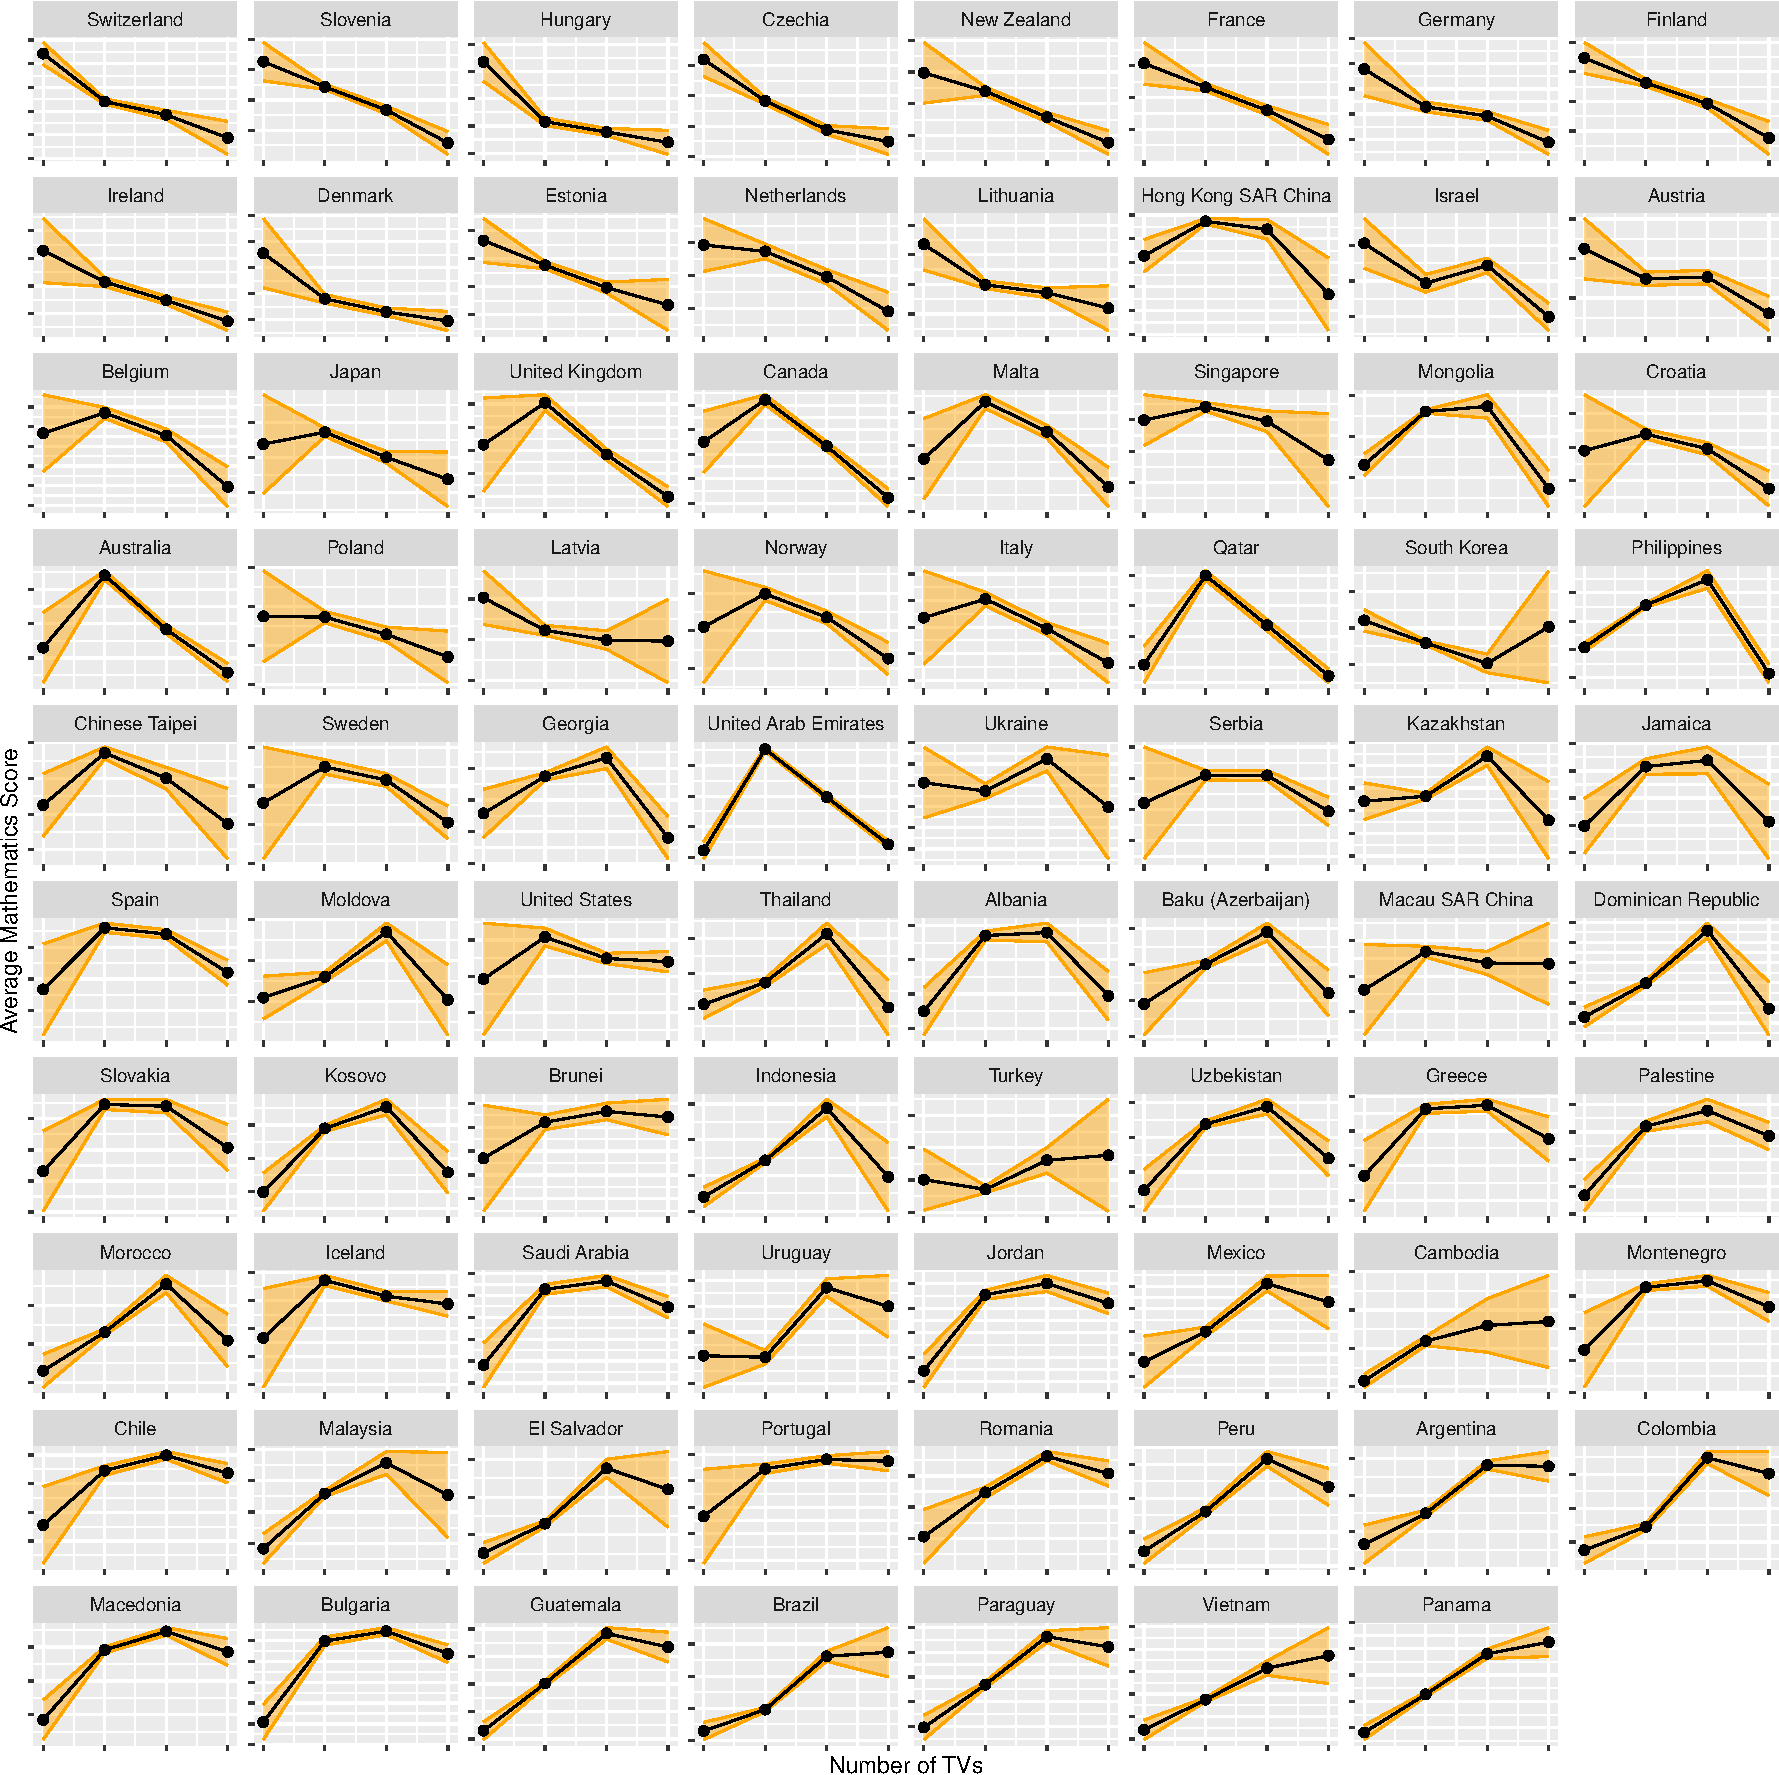
\includegraphics[width=1\textwidth,height=\textheight]{Learningtower_Rpackage_files/figure-pdf/fig-tvplot-1.pdf}

}

\caption{\label{fig-tvplot}Relationship between number of TVs in a
household and average math scores across countries. Number of TVs ranges
from 0 to 3 or more. The orange bands indicate 95 percent standard
confidence intervals. The impact of television on student performance is
a contentious issue. It is interesting that in some countries for
example in South Korea's effect appears to be positive, but in other
countries like Poland and Germany there is a decline in average math
scores.}

\end{figure}%

\begin{figure}[H]

\centering{

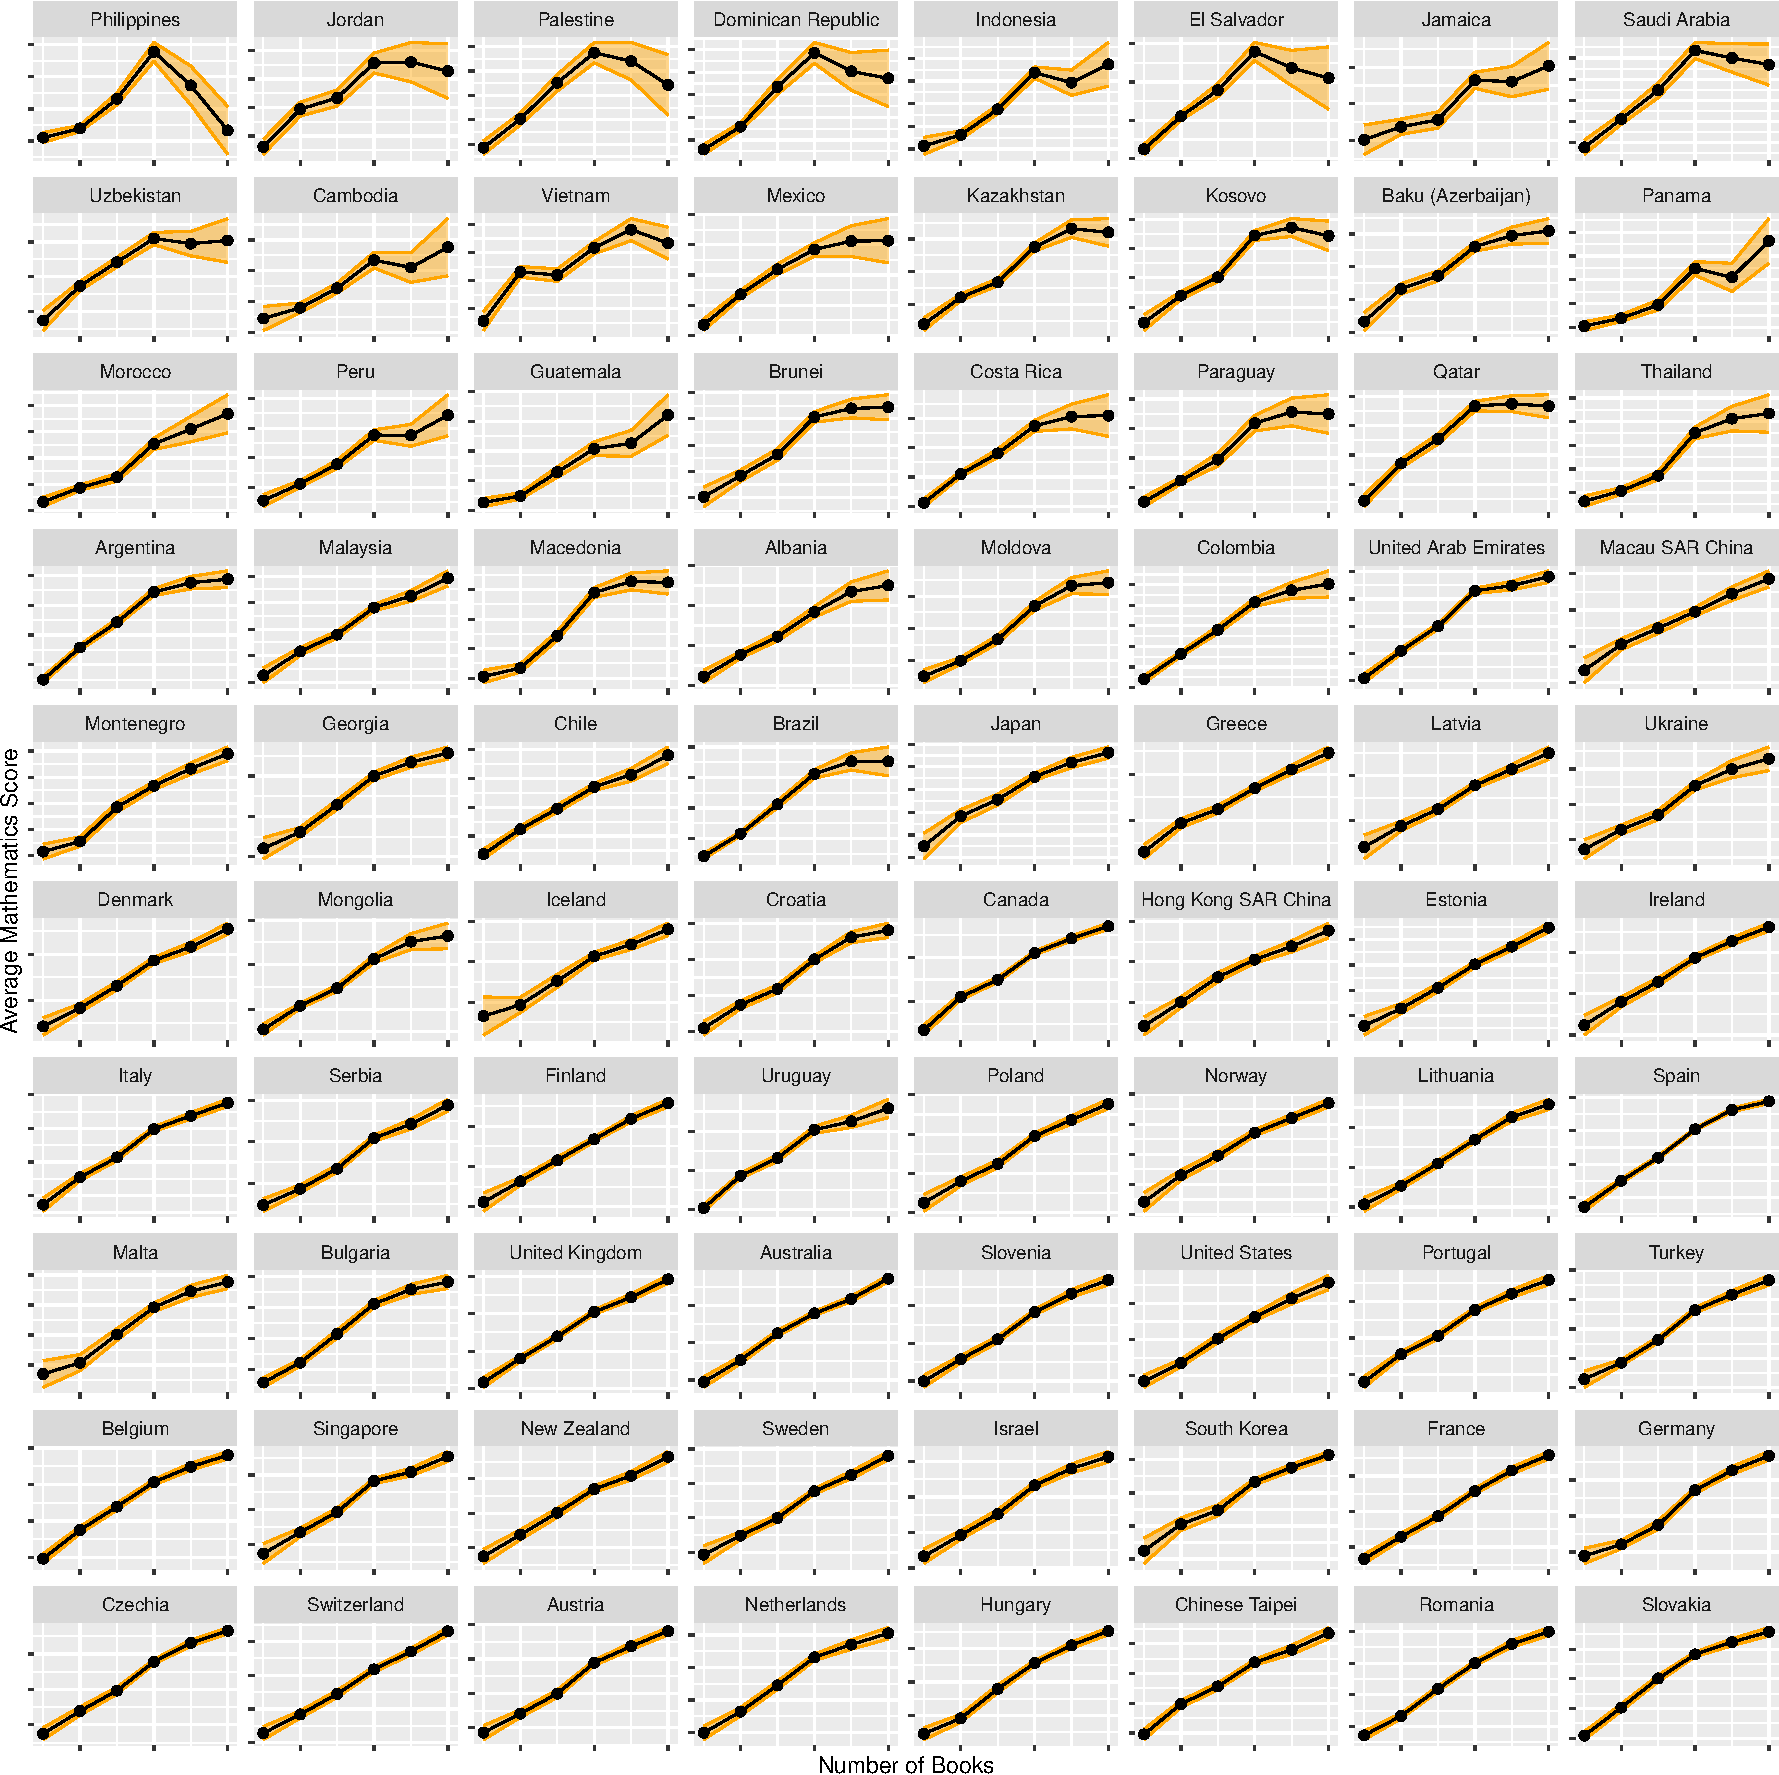
\includegraphics[width=1\textwidth,height=\textheight]{Learningtower_Rpackage_files/figure-pdf/fig-bookplot-1.pdf}

}

\caption{\label{fig-bookplot}Impact of the number of books on average
math score. Number of books ranges from 0 to 500 and more. 95 percent
standard confidence bands shown in orange. Math scores generally
increase as the number of books increases. Averages for some countries
at the higher number of books are less reliable, and hence the decline
reflects more that there are few households with this many books than a
true decline.}

\end{figure}%

\begin{figure}[H]

\centering{

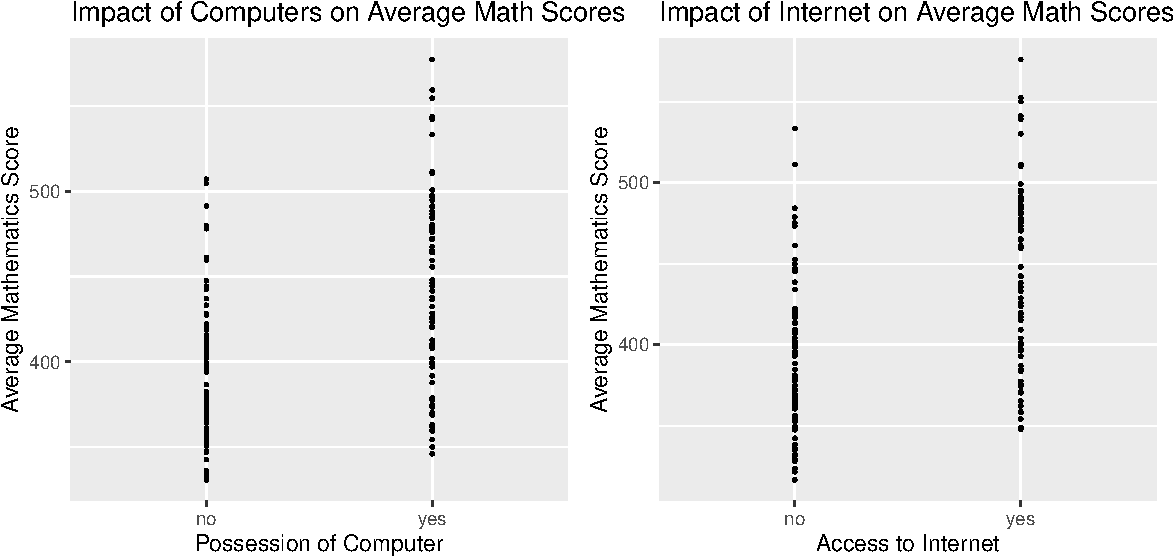
\includegraphics[width=1\textwidth,height=\textheight]{Learningtower_Rpackage_files/figure-pdf/fig-compintplot-1.pdf}

}

\caption{\label{fig-compintplot}Computers and the Internet are two of
the most important inventions in the history of technology. In this
figure, we observe the impact of owning a computer and having access to
the internet on 15-year-old students all over the world. A remarkable
finding from the plot is that all nations have higher scores in student
performance when they own a computer and have access to the internet.}

\end{figure}%

\subsection{Temporal Analysis}\label{temporal-analysis}

\subsubsection{Pandemic effects}\label{pandemic-effects}

\begin{figure}[H]

\centering{

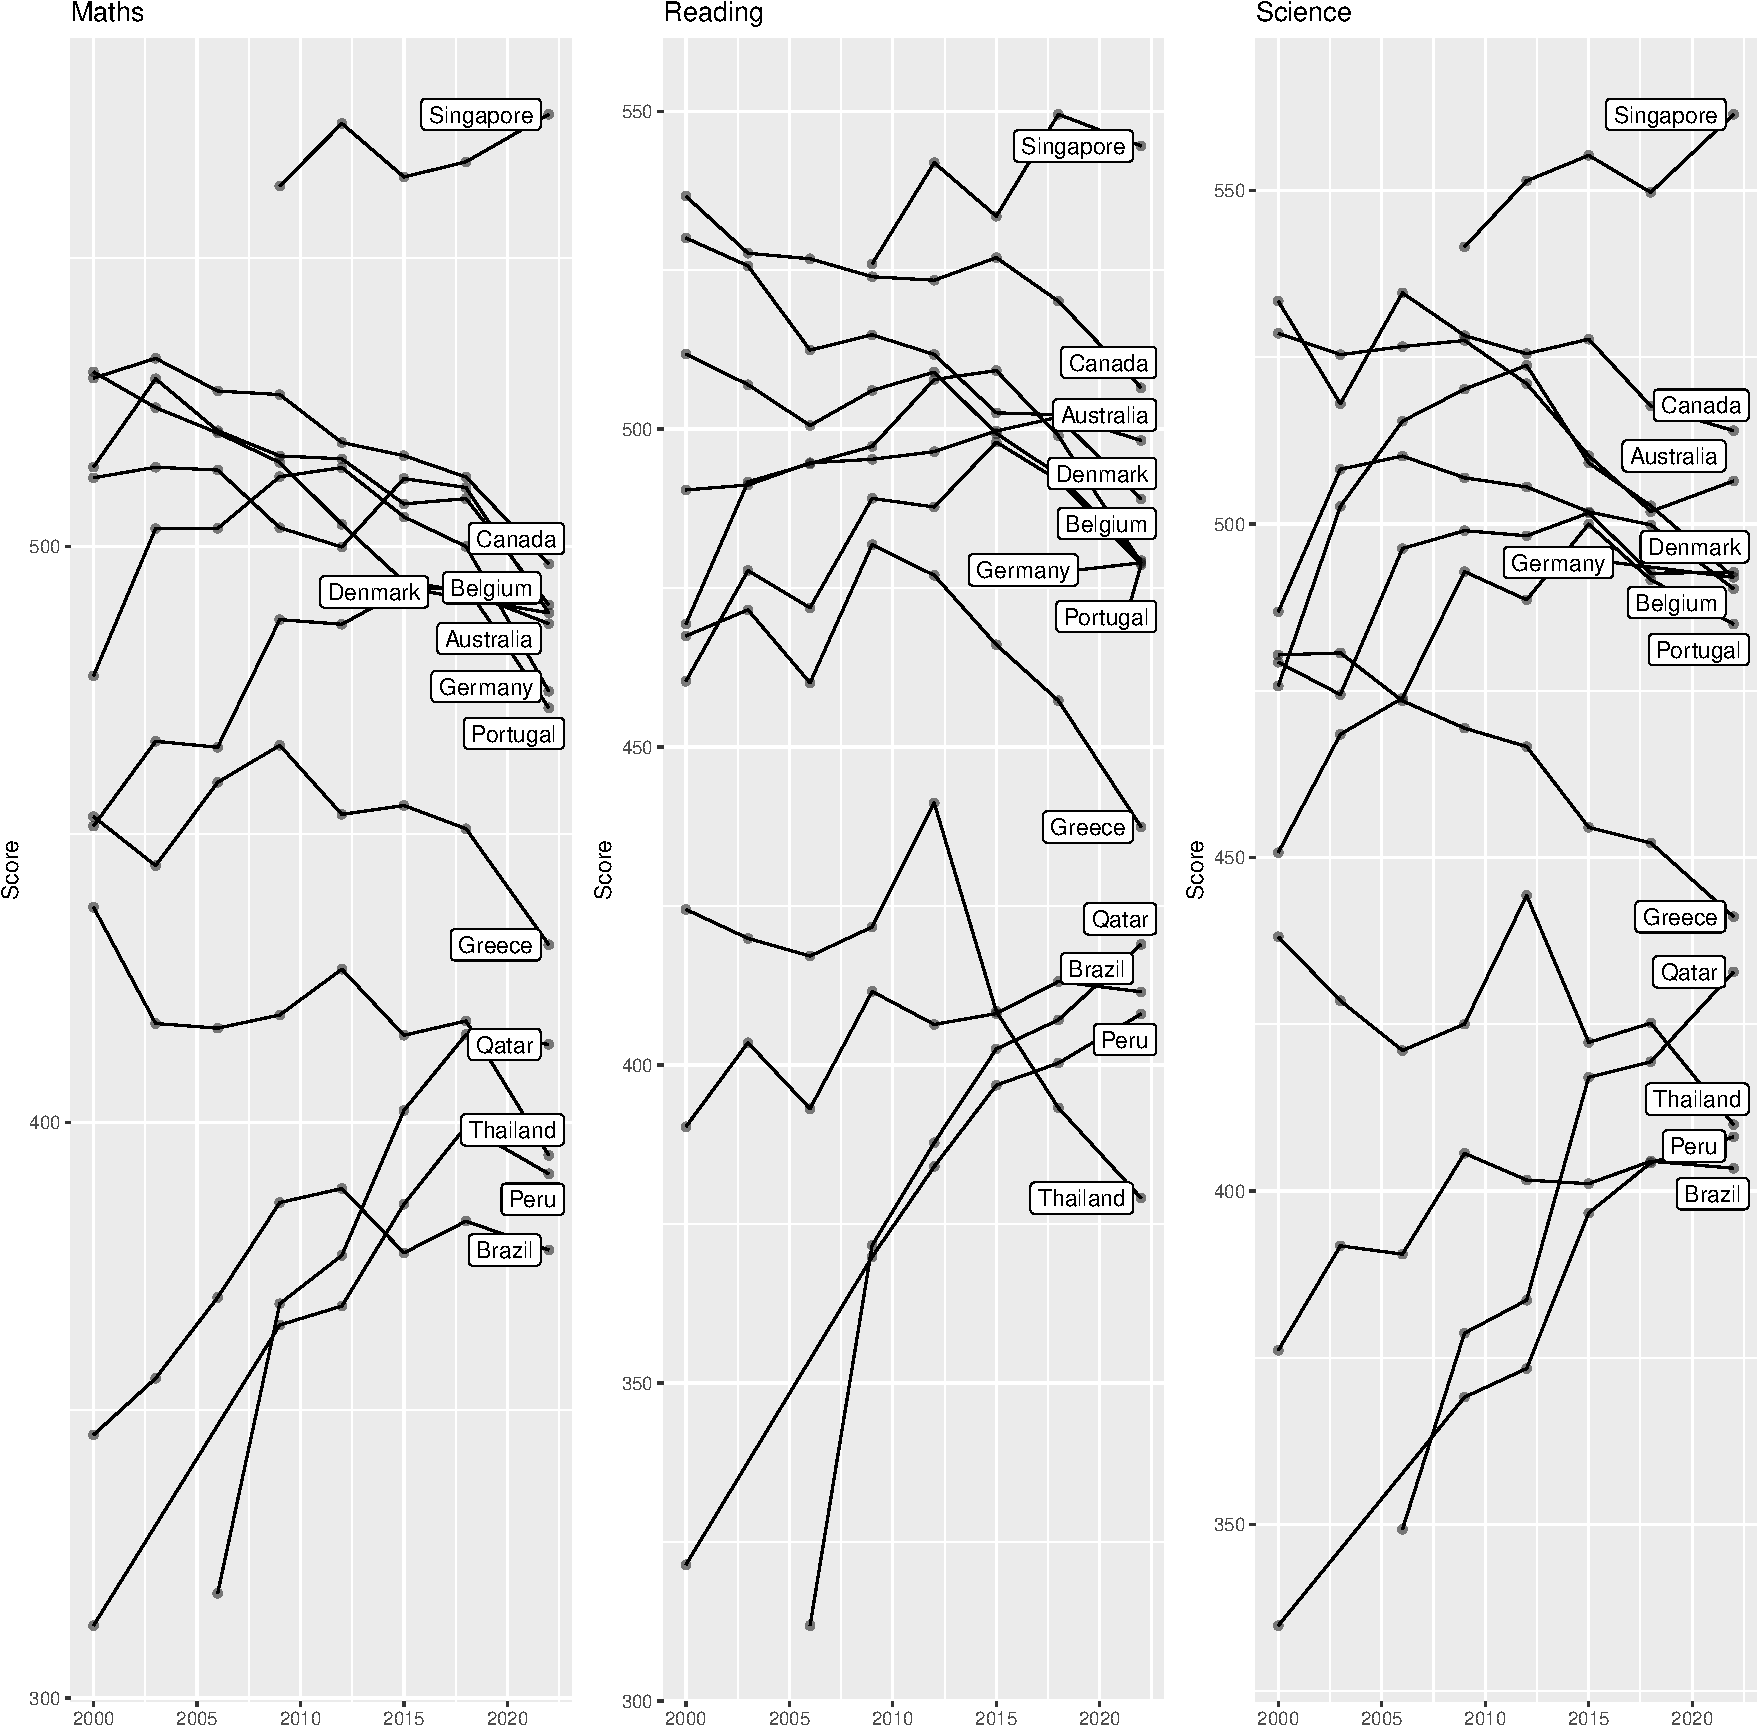
\includegraphics[width=1\textwidth,height=\textheight]{Learningtower_Rpackage_files/figure-pdf/fig-bsplot-1.pdf}

}

\caption{\label{fig-bsplot}Temporal patterns in math, reading, and
science in a variety of countries. The highlighted countries in the
chart help us infer Australia's performance in contrast to the other
countries; we can see that Australia's scores have always been among the
highest in the PISA survey throughout all years.}

\end{figure}%

\subsubsection{Gender Gaps Across Subjects and
Years}\label{gender-gaps-across-subjects-and-years}

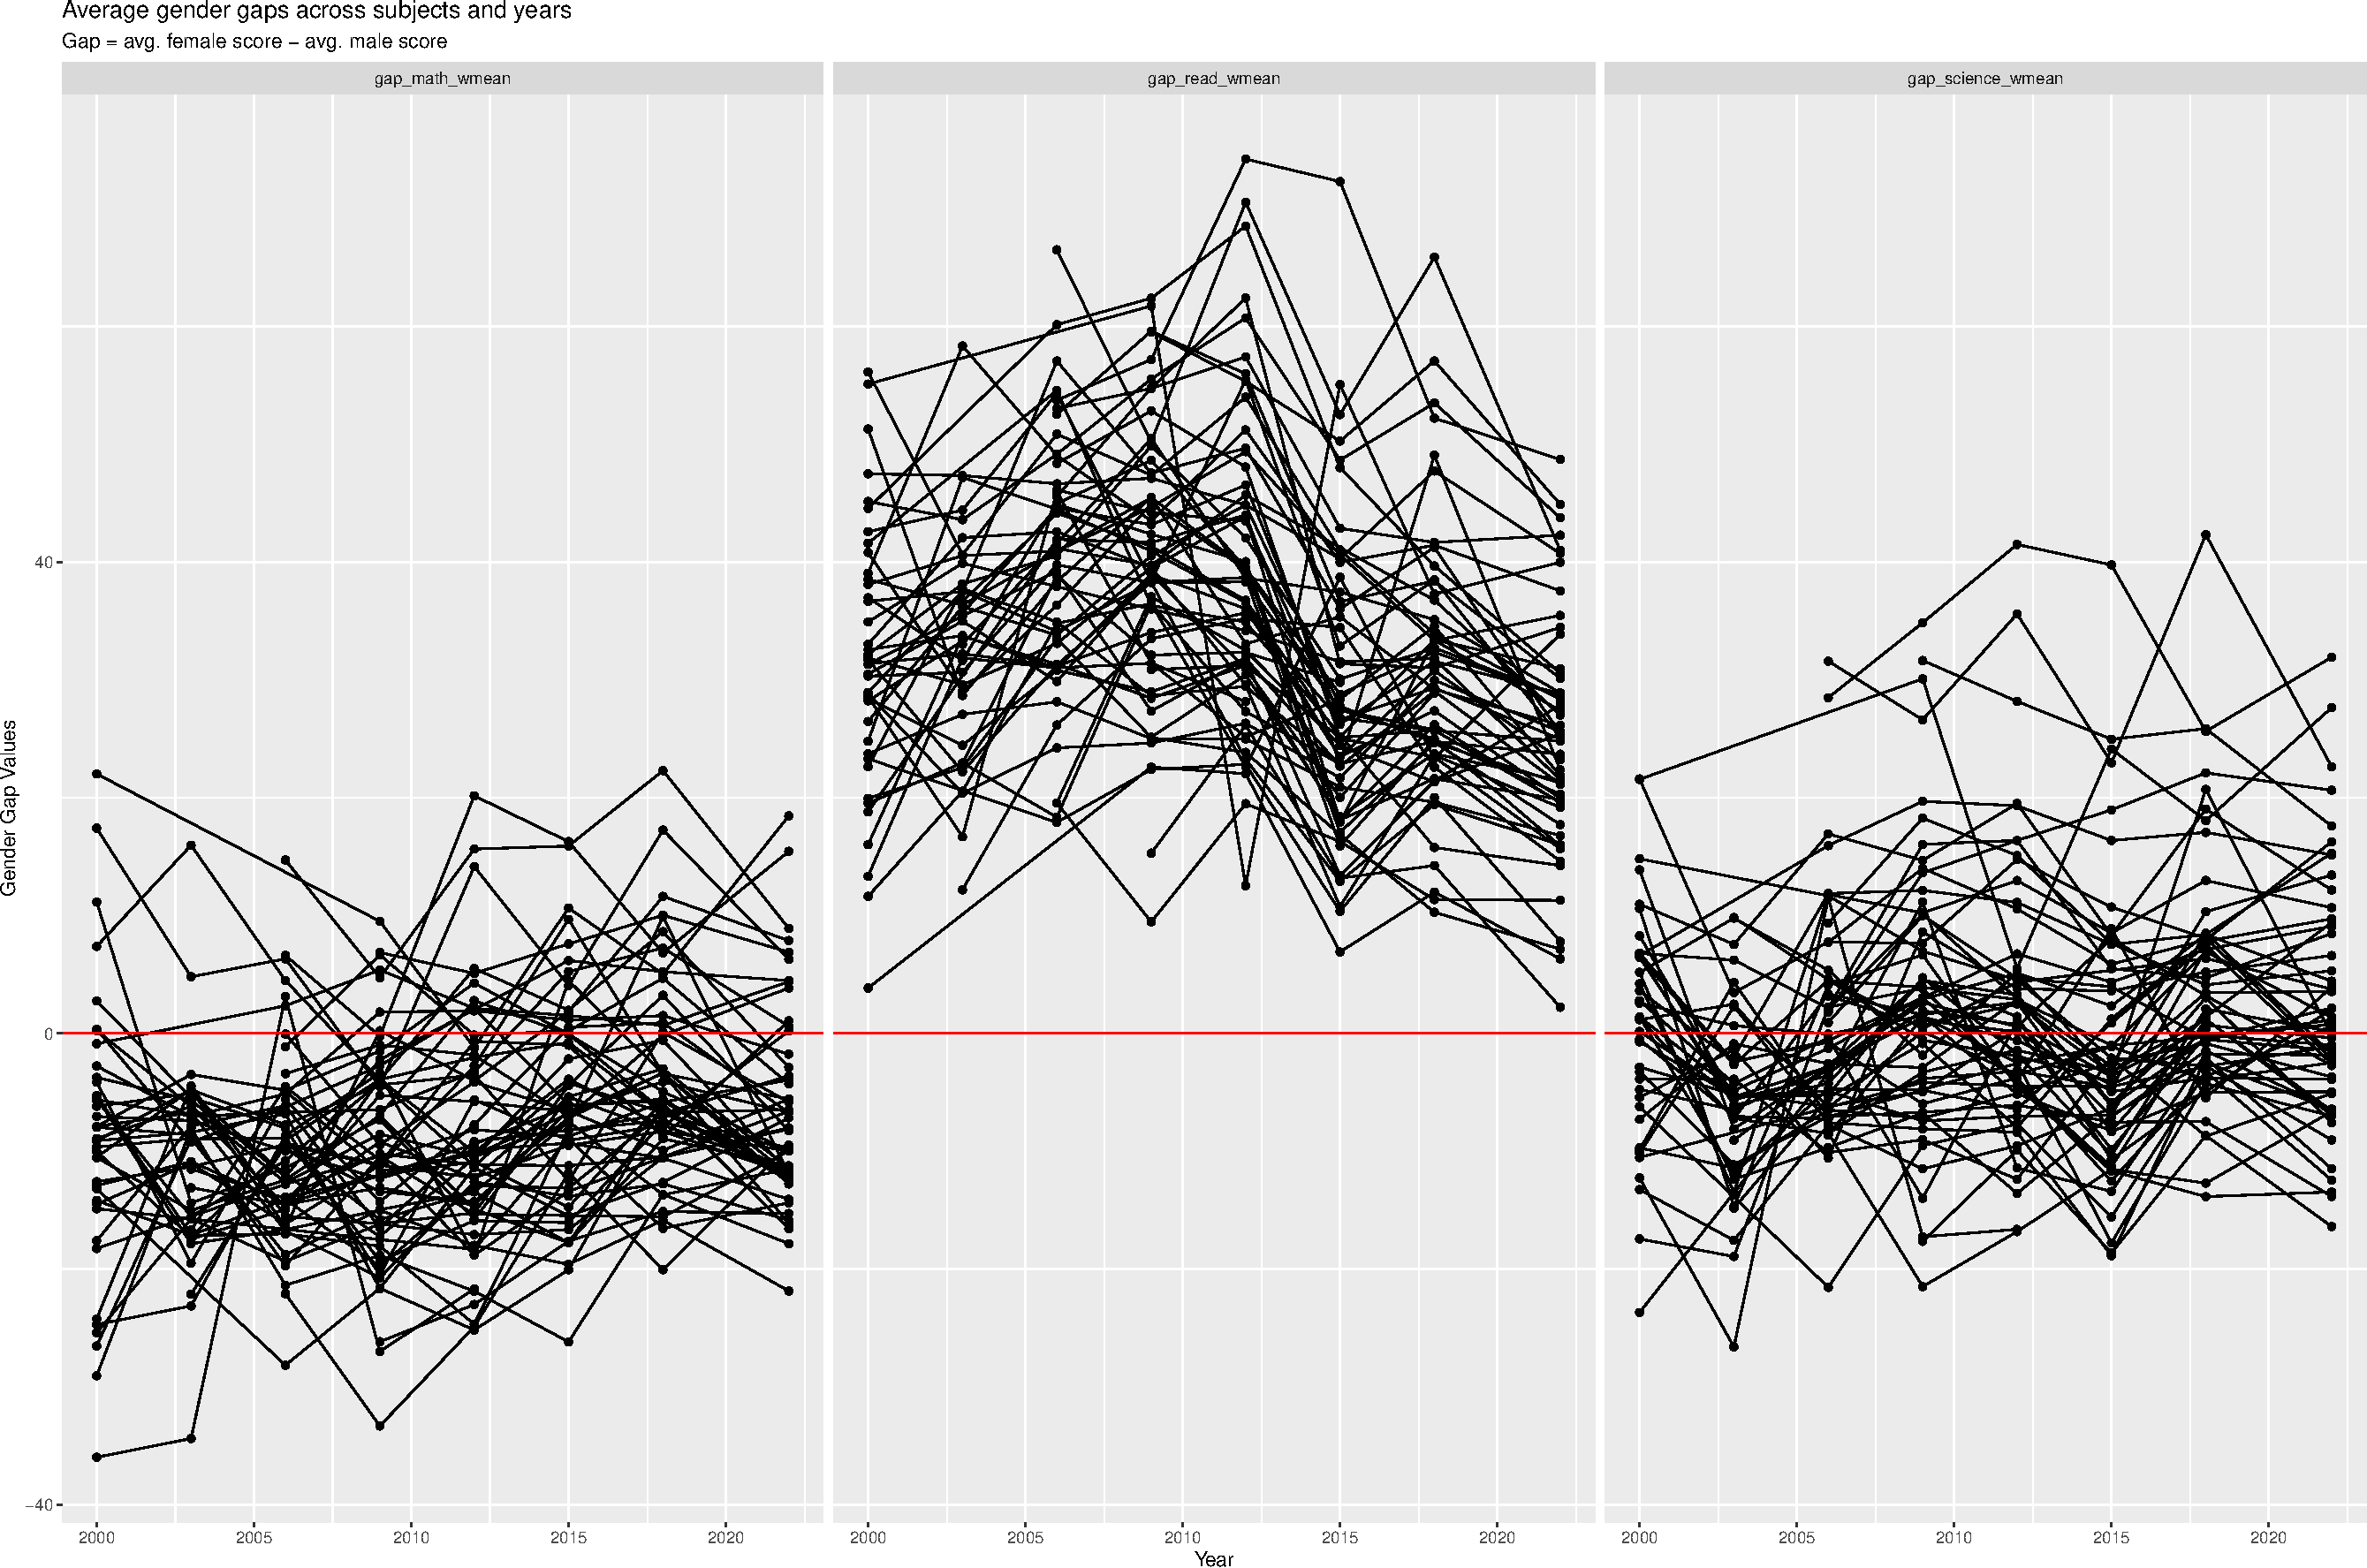
\includegraphics{Learningtower_Rpackage_files/figure-pdf/unnamed-chunk-21-1.pdf}

\subsubsection{Highlighting Key
Countries}\label{highlighting-key-countries}

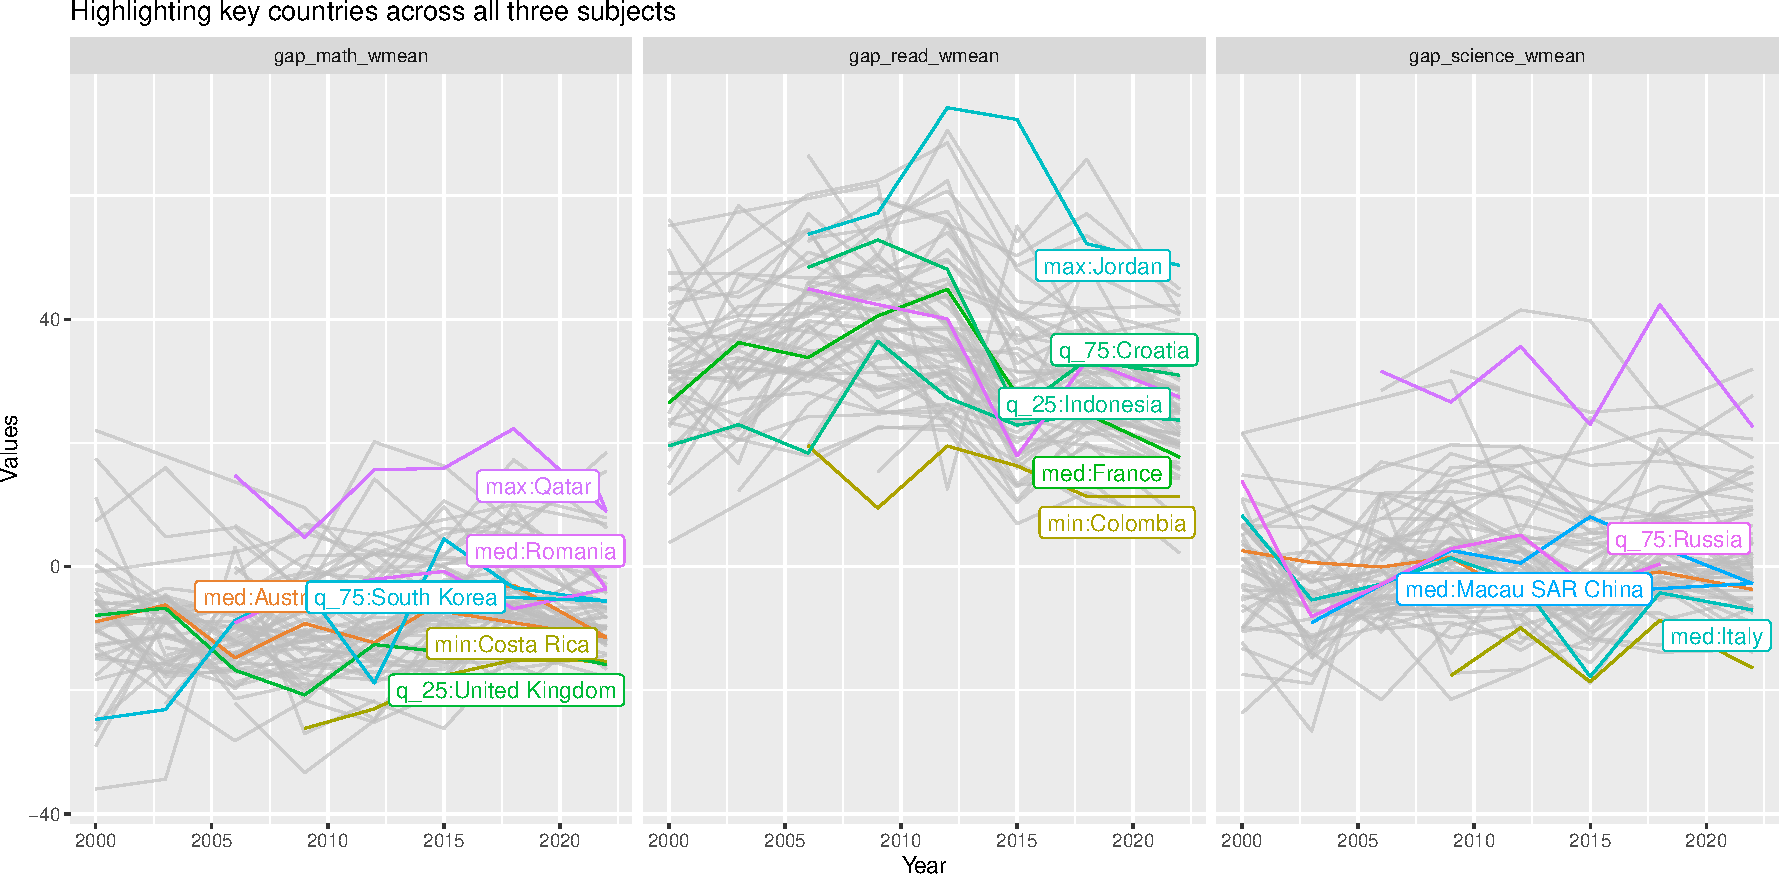
\includegraphics{Learningtower_Rpackage_files/figure-pdf/unnamed-chunk-22-1.pdf}

\section{Discussion}\label{discussion}

\subsection{Limitations}\label{limitations}

\begin{itemize}
\item
  Size limitation on CRAN packages: The data size would be bigger if
  keep uploading the newest data, so further curation process of data
  should be considered, or explore alternative data compression for the
  datasets.
\item
  Variables Consistency: The construction of questionnaire would be
  different every survey, as well as the coding mechanism of the
  original dataset, so curation process must be examined everytime to
  ensure the consistency of variables.
\end{itemize}

\section{Conclusion}\label{conclusion}

An important improvement is the addition of the 2022 PISA data to the
learningtower R package, which provides current insights from student
and school statistics. By providing a thorough grasp of student
performance, school characteristics, and the factors impacting learning
outcomes, this update facilitates a deeper comprehension of global
educational dynamics. The program facilitates cross-country comparisons
and rigorous longitudinal analysis by guaranteeing consistency across
datasets from 2000 to 2022.

The learningtower package's improvements give educators, researchers,
and policymakers useful tools for evaluating and enhancing educational
institutions. The package promotes data-driven initiatives to address
educational issues and advance fairness by providing a comprehensive
strategy that integrates student and school data. Learningtower will
remain a vital tool for expanding our knowledge of global educational
trends and promoting significant learning gains as long as it is updated
to include upcoming PISA statistics.

\section{Reference}\label{reference}

\subsection{Git respository of the
report}\label{git-respository-of-the-report}

https://github.com/Shabarish161/Learningtower\_Rpackage


\printbibliography


\end{document}
